% !TEX root = ../../document.tex

\documentclass{subfiles}

\begin{document}

  \chapter{Implementación y Resultados}
  \label{chap:implementation_results}

    \section{Introducción}
    \label{sec:implementation_results_introduction}

      \paragraph{}
      Hasta ahora, el objetivo principal de este documento se ha orientado en la descripción y análisis del problema \emph{Dial-a-Ride} desde una perspectiva principalmente teórica, incluyendo una descripción detallada centrada en la \emph{Formulación del Problema} en el \cref{chap:formulation} así como un análisis sobre los \emph{Métodos de Resolución} disponibles para el problema en el \cref{chap:solving}. A lo largo de dichos capítulos se ha podido apreciar tanto las dificultades inherentes al propio problema por las características propias que este presenta, tales como el tiempo máximo de duración de trayecto (calidad del servicio), así como otros factores relacionados con la complejidad computacional de resolver un problema de esta naturaleza (englobado en la clase de problemas \emph{NP}).

      \paragraph{}
      Sin embargo, el este capítulo representa un cambio de perspectiva del problema, estando centrado más en los detalles de implementación de una biblioteca bautizada como \texttt{jinete} y desarrollada sobre el lenguaje \emph{Python}, cuyo enfoque consiste en proporcionar una serie de herramientas que sobre las cuales ser construir métodos de resolución de problemas de rutas. En una primera implementación, el desarrollo de dicha biblioteca se ha orientado principalmente hacia la resolución del problema \emph{Dial-a-Ride} mediante una estrategía inspirada en la metaheurística \emph{GRASP} descrita en el \cref{sec:solving_grasp}. En el \cref{sec:implementation} se incluye una descripción detallada acerca de la implementación realizada, así como las ideas en que ha inspirado la misma.

      \paragraph{}
      Para demostrar el funcionamiento de la implementación realizada, así como proporcionar una ejemplificación de su uso, se han utilizado una serie de instancias del problema disponibles en la web de manera pública, que han sido utilizados a modo de \emph{benchmark} en una gran cantidad de documentos científicos de gran reconocimiento. El \cref{sec:results} se destina a dicho cometido.

      \paragraph{}
      Por último, en el \cref{sec:implementation_results_conclusions} se expone una conclusión relacionada con el proceso de implementación de estrategias de resolución del problema \emph{Dial-a-Ride}, indicando las principales debilidades de la implementación actual, así como sus posibles puntos de mejora.

    \section{Implementación}
    \label{sec:implementation}

      \paragraph{}
      Tal y como se menciona en la introducción del capítulo, este apartado se dedica integramente a comentar la implementación realizada durante el desarrollo de este trabajo, donde se describen de manera detallada desde las decisiones tomadas de alto nivel (en el \cref{sec:implementation_high_level}) en la que se comentan aspectos como el lenguaje de implementación elegido o la metaheurística implementada de manera concreta, continuando con una descripción acerca de las decisiones tomadas en lo relacionado con un nivel de más bajo (en el \cref{sec:implementation_low_level}) en el que se describen los módulos más relevantes así como algunas de las decisiones algorítmicas tomadas. Además, a lo largo de la descripción se trata de presentar una breve discusión acerca de las distintas decisiones de diseño tomadas a lo largo del proceso, tratando de destacar las principales ventajas e inconvenientes de cada una de ellas.

      \subsection{Decisiones de Alto Nivel}
      \label{sec:implementation_high_level}

        \paragraph{}
        El objetivo principal de la implementación realizada puede ser resumido en una frase: \textbf{Razonar en detalle la implementación de un sistema capaz de generar soluciones válidas (y lo más cercanas al valor óptimo posible) para el problema Dial-a-Ride}. Sin embargo, tal y como se puede apreciar, dicha frase es de carácter muy general y puede abarcar una gran cantidad de tareas a realizar, desde el estudio y adaptación de restricciones definidas como desigualdades en un modelo lineal para que estas después sean implementadas sobre uno de los sistemas comerciales más populares como \texttt{FICO Xpress Mosel} o \texttt{IBM CPLEX}, hasta el diseño de alguna metaheurística por completo en algún lenguaje como \texttt{C++}, \texttt{Rust} o \texttt{Python}. Tal y como se puede intuir, cualquiera de estas tareas puede llegar a ser por si sola motivo de una trabajo de tesis con el conveniente grado de profundización en la materia. Sin embargo, dado que en este caso el trabajo se ha llevado a cabo sobre el contexto de un \emph{Trabajo de Fin de Grado} (con sus correspondientes limitaciones temporales), la implementación que se ha llevado a cabo consiste en una tarea intermedia entre estos dos caminos, a costa de un menor grado de profundidad en cada uno de ellos, pero que ha permitido conocer las complicaciones reales que la literatura relacioanda con el problema \emph{Dial-a-Ride} pretende resolver para que las soluciones alcanzadas sean aplicables sobre situaciones reales y no queden en meros ejercicios teóricos.

        \paragraph{}
        Una de las decisiones importantes dede el punto de vista de los objetivos de la implementación es elegir el lenguaje sobre el cuál se va a llevar a cabo. El motivo de sobre la relevancia de dicha decisión desde el punto de vista del objetivo de la misma está intimamente relacionada con el alcance del trabajo. En este caso, los principales factores que han influido en dicha decisión han sido la capacidad de generar una implementación relativamente elaborada en un tiempo relativamente reducido, la experiencia en el propio lenguaje y el ecosistema de herramientas relacionadas compatibles con el mismo. Por contra, se han obviado otros factores como el grado de eficiencia del mismo (el cual es muy importante en este tipo de sistemas) pero que se ha dejado en un segundo nivel por la naturaleza didáctica del mismo. Tras tener en cuenta todos estos factores, la decisión tomada ha sido la de elegir \texttt{Python 3} \cite{rossum1995python} como lenguaje sobre el cual realizar la implementación. Este proporciona la capacidad de llevar a cabo implementaciones relativamente grandes en un periodo de tiempo inferior a la que se requeriría por otros lenguajes más verbosos como \texttt{Java} o \texttt{C++} además de proporcionar una sintaxis con una alta legibilidad, lo cual es una factor muy beneficioso en el contexto de los métodos de resolución de problemas como el \emph{Dial-a-Ride}. Otro de los factores es la experiencia adquirida sobre este lenguaje, lo cual es un factor muy facilitador. Sin embargo, la elección escogida también presenta desventajas, sobre todo de escalabilidad a largo plazo y extensión de la misma desde un contexto didáctico hacia otro más aplicable a situaciones reales. Esto se debe a la ineficiencia que este lenguaje presenta frente a otros con una interfaz a un nivel más bajo, que (a costa de una mayor complejidad de desarrollo) son algunos órdenes de magnitud más rápidos. Este es uno de los factores que se comentarán en los próximos pasos, destacando la posibilidad de llevar a cabo una reimplementación de la biblioteca actual sobre el lenguaje \texttt{Rust}.

        \paragraph{}
        En relación con las ideas expuestas en los anteriores párrafos, y obviando la decisión sobre el lenguaje sobre el cuál se ha llevado a cabo la implementación, uno de los factores más importantes para entender la implementación realizada ha sido la naturaleza de la misma. En este caso, en lugar de tratar de llevar a cabo el desarrollo de una serie de ficheros que permitan resolver únicamente el problema \emph{Dial-a-Ride}, sin tener en cuenta las posibles variantes que este pueda llegar a tener, así como las partes en común que distintos métodos de resolución compartan, en este caso se ha primado el análisis de dichas partes. De este modo se ha conseguido alcanza una estructura en forma de biblioteca, la cual se caracteriza por proporcionar una interfaz de utilización externa, sobre la cuál definir por ejemplo la manera de \say{cargar} el fichero de entrada que contiene la entrada del problema así como la estrategia de resolución que se desea utilizar e incluso el modo en que se exportarán los resultados. Por otra parte, se ha tratado de mantener oculta al exterior toda la complejidad inherente a este tipo de problemas de optimización, lo cuál es un punto a favor para ser utilizado por personas que no sean lo suficentemente expertas en la materia. En relación con la naturaleza en forma de biblioteca, también se ha tratado de priorizar la estructura de composición en los métodos de resolución. Es decir, en lugar de proporcionar una serie de implementaciones bien definidas, se ha pretendido proporcionar una interfaz extensible y que favorezca la composición. Esto se puede apreciar en situaciones como la definición (o eleeción) de los criterios de selección en ciertas estrategias de naturaleza \emph{greedy} o la capacidad de componer de manera personalizada distintas metaheurísticas que requieren de fases de inserción llevadas a cabo por otras posibles heurísticas (o metaheurísticas). Cuando se ejemplifique su utilización esto se podrá apreciar de manera más clara.

        \paragraph{}
        Una de las partes más importantes a la hora de estudiar \emph{problemas de rutas} como el \emph{Dial-a-Ride} consiste en el análisis del mismo desde un pusto de vista más teórico. Uno de los caminos para llevar a cabo dicha tarea es el estudio de la formulación del mismo como \emph{problema de programación lineal} donde, cómo se ha indicado en el \cref{sec:formulation_real_time}, es necesario definir tanto la naturaleza de una serie de variables de decisión, como las restricciones que estas presentan entre si, como la función objetivo (en este caso de minimización). Para que dicho ejercicio de estudio teórico del problema sea completo, también es una buena práctica la de implementarlo en uno de los solvers de propósito general más populares como \texttt{CPLEX} o \texttt{Mosel} de tal manera que se puedan apreciar los resultados así como comprender las dificultades computacionales desde una perspectiva mucho más cercana. Sin embargo, en este trabajo se ha seguido un enfoque ligeramente distinto para tratar de mantener lo más unificada posible la implementación llevada a cabo en \texttt{Python} con la obtenidas por distintos solvers. Para ello, se ha utilizado una heramienta desarrollada por la \emph{COIN-OR Foundation} cuyo cometido es el de proporcionar una interfaz de comunición entre \texttt{Python} y los solvers más conocidos, la cual se conoce como \texttt{PuLP} \cite{mitchell2011pulp}. Para desenpeñar su tarea, esta biblioteca proporciona una interfaz sobre la cual llevar a cabo la formulación del problema a partir de sentencias como \texttt{[TODO]} (para definir el problema), \texttt{[TODO]} (para definir variables), \texttt{[TODO]} (para definir restricciones) o \texttt{[TODO]} (para proceder a la optimización del problema). Internamente, dicha biblioteca es capaz de comunicarse con una gran cantidad de solvers (en el apartado de resultados se incluye una breve comparativa entre estos). Posteriormente, se ha añadido un nivel de abstracción superior capaz de convertir los resultados de la formulación lineal en conceptos relacionados con los problemas de rutas como \emph{Vehículo}, \emph{Ruta} o \emph{Viaje}. De esta manera es sencillo realizar comparaciones entre métodos de resolución basados en heurísticas frente a otros basados en métodos exactos, además de compartir la misma implementación tanto para la lectura de los datos como para exportación de los resultados.

        \paragraph{}
        Hasta ahora se ha comentado el objetivo de la implementación realizada desde el punto de vista de algunas de las decisiones de implementación tomadas a priori (tales como el lenguaje utilizado o la filosofía seguida durante el proceso), sin embargo, aún no se ha expuesto en detalle la problemática concreta que dicha implementación es capaz de resolver, ni la estrategia seguida para llevarlo a cabo. En cuanto a la problemática concreta que esta biblioteca trata de resolver, es fácil intuir (por ser el tema principal del trabajo) que se trata de ser capaz de generar soluciones factibles para el problema \emph{Dial-a-Ride}. Por contra, la segunda parte de la cuestión requiere de una clarificación en mayor profundad: Por una parte, esta implementación es capaz de generar soluciones basándose en métodos de resolución de problemas lineales gracias a la formulación del problema \emph{Dial-a-Ride} de dicha forma, tal y como se ha comentado en el párrafo anterior. Por otro lado, actualmente la biblioteca es capaz de generar soluciones siguiendo una estrategia metaheurística de naturaleza \emph{GRASP}, lo cual implica, entre otros, la implementación de una algoritmo de inserción \emph{Greedy}, una heurística de \emph{Búsqueda Local} capaz de mejorar una solución previamente generada en este caso, por la estrategia \emph{Greedy}, y la propia lógica de control de la estrategia \emph{GRASP}, encargada de controlar si se cumplen las condiciones suficientes para llevar a cabo un nuevo ciclo de mejora de la solución actual así como otros aspectos relacionados. Es importante remarcar que todos estos módulos pueden ser utilizados añadiendo distintas puntos de aleatoriedad (para así tratar de reducir el alcanzamiento de mínimos locales \say{sin salida}). De forma complementaria a la capacidad de añadir una módulo de aleatoriedad, también se incluye la capacidad de apoyarse en un \say{generaror de múltiples soluciones} que es capaz de integrarse en cualquier fase del proceso. Posteriormente se detallará más este módulo, el cual se encarga de orquestar la generación de soluciones con distintas módulos de aleatoriedad y posteriormente seleccionar cual de todas ellas debe continuar con el proceso de optimización.

        \paragraph{}
        A lo largo de este apartado, se ha llevado a cabo una descripción acerca de las distintas decisiones tomadas a lo largo del desarrollo de la implementación desde una perspectiva externa, exponiendo las razones y tratando de comentar otras alternativas a las finalmente escogidas. Estas han sido desde comentar el lenguaje utilizado, la naturaleza de la implementación, su conexión con los métodos de resolución basados en formulación como problema de programación lineal, hasta el alcance de la metaheurística implementada de manera demostrativa.

        \paragraph{}
        Por otro lado, es importante remarcar también las decisiones tomadas en lo relativo al desarrollo de software muy importante en casos como los métodos de resolución en \emph{problemas de optimización combinatoria}, donde el gran peso de la módulo algorítmica (sobre todo en lo relacionado con \emph{metaheurísticas}) es crucial para alcanzar los resultados deseables. Dicho razonamiento se llevará a cabo a lo largo del próximo apartado.

      \subsection{Decisiones de Bajo Nivel}
      \label{sec:implementation_low_level}

        \paragraph{}
        En este apartado se pretende llevar a cabo una descripción desde un punto de vista más técnico y detallado sobre las decisiones tomadas a lo largo de la implementación de la biblioteca en cuestión. Para ello, se dedican distintos sub-apartados a cada uno de los factores más relevantes a tratar. En primer lugar, se ilustra la organización de la biblioteca, dividida en módulos en el \cref{sec:implementation_components}. A continuación, se comenta el modelo de datos definido para resolver el problema, el cual guarda una estrecha correlación con el definido en el \cref{chap:formulation} donde se lleva a cabo una breve descripción de la nomenclatura utilizada. Finalmente, se trata de profundizar con un mayor nivel de detalle en cada uno de los módulos anteriormente indicados a lo largo de los \cref{sec:implementation_components_data_loading,sec:implementation_components_optimization,sec:implementation_components_exportation}.

        \subsubsection{Organización Basada en Módulos}
        \label{sec:implementation_components}

          \paragraph{}
          La estructura en que se ha organizado la biblioteca se ha definido tratando de tener en cuenta la facilidad para ser extendida y ampliada con el paso del tiempo, de tal manera que sea sencillo incluir tanto nuevas estrategias de resolución más sofisticadas, como la capacidad de poder modelar otros problemas de rutas de vehículos de una manera sencilla. Para ello, se ha tratado de prestar especial importancia al desacoplamiento entre los distintos elementos que la componen así como la decisión de dar un sentido único y bien definido a cada uno de ellos.

          \paragraph{}
          Estos conceptos se entienden de manera mucho más sencilla a través de un ejemplo: en la implementación llevada a cabo, el módulo encargado de proceder a la carga de datos se considera desacoplado del resto puesto que la única comunicación que soporta consiste en las peticiones para llevar a cabo la carga de datos, así como la de suministrar estos en un formato ya adaptado para que pueda ser utilizado por el resto de la biblioteca (el cual se comenta en el \cref{sec:implementation_components_data_model}). En cuanto al sentido único que este módulo presenta, dicha característica consiste en que es fácil comprender la función que desempeña, lo cual facilita el proceso futuro de crear nuevas versiones de dicho módulo para que, por ejemplo, en lugar de cargar los datos desde un fichero concreto alojado en la máquina en cuestión, este sea capaz de recibirlo desde una dirección específica de internet u otro tipo de estrategias de definición más complejas como la carga desde una base de datos. Dichas capacidades de extensión permiten integrar la implementación realizada en sistemas reales de una forma muy sencilla y mantenible.

          \begin{figure}[ht]
            \centering
            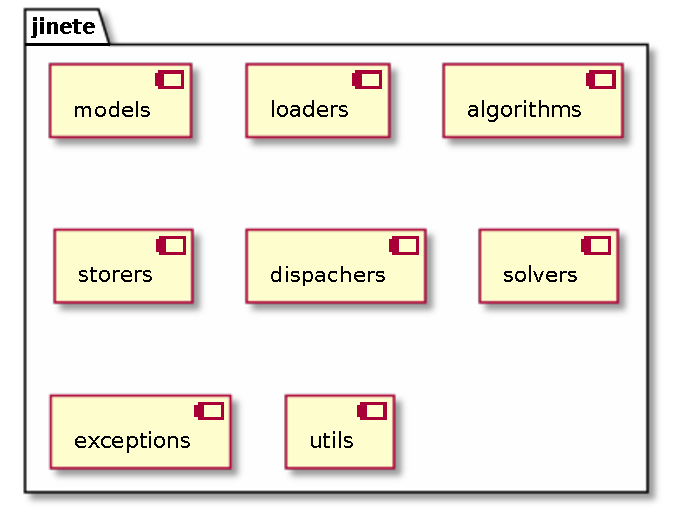
\includegraphics[width=0.5\textwidth]{modules-overview}
            \caption{Diagrama basado en módulos de la biblioteca \texttt{jinete}}
            \label{img:modules_overview}
          \end{figure}

          \paragraph{}
          En cuanto a la organización completa de la biblioteca, esta se divide en 4 módulos principales, que además de apoyarse entre si, utilizan otros módulos de menor tamaño tal y como se comentará a lo largo del apartado. En la \cref{img:module_overview} se incluye una representación gráfica de estos. En cuanto a los módulos principales, a continuación se proporciona una breve descripción acerca de cada uno de ellos (el orden en que se describen se corresponde con el flujo natural en que estos se interrelacionan lo cual pretende servir para clarificar aún más su funcionamiento):

          \begin{itemize}
              \item \texttt{models}: Es el encargado de definir las entidades que representan los distintos elementos necesarios para modelar los distintos problemas de rutas, entre los que se encuentran clases como \texttt{Vehicle}, \texttt{Route} o \texttt{Stop}. Dichas entidades son las encargadas de poseer la información acerca de las restricciones del problema (como por ejemplo la ventana temporal en que es factible llevar a cabo parada de recogida para un determinado viaje), pero además se encargan de recoger el estado tras cada etapa de ejecución del proceso de optimización (como por ejemplo el instante de tiempo en que se encuentra un determinado vehículo al haber realizado un secuencia concreta de viajes).Dichas entidades representan además un \say{contrato} entre el resto de módulos y submódulos de la biblioteca, lo cual es una de las herramientas que permite hacer más mantenible y ampliable la implementación realizada. Posteriormente se detalla de manera más precisa, pero a modo de ejemplo es fácil apreciar las ventajas de definir una entidad común \texttt{Route} que pueda ser utilizada por las distintas estrategias de optimización sin que estas requieran de otra característica adicional, lo que permite flexibilizar la capacidad de combinación y/o composición de dichas estrategias. En el \cref{sec:implementation_components_data_model} se lleva a cabo una descripción más detallada acerca del módulo.

              \item \texttt{loaders}: Tal y como se ha comentado anteriormente a modo de ejemplo, la responsabilidad de este módulo consiste en ser capaz de cargar los datos desde una fuente de datos externa sobre la cual estos están definidos siguiendo un determinado formado posiblemente distinto del deseado, el cual consiste en las definidas por el módulo \texttt{models}. De esta manera, es posible aplicar indistintamente las distintas técnicas y herramientas implementadas en la biblioteca ignorando la estructura de los datos originales. Más adelante se describe de manera más detallada, sin embargo es interesante remarcar que en dicha tarea hay dos dimensiones principales: la \say{lectura} de la fuente de datos, la cual puede ser desde la carga de un fichero hasta el acceso a una base de datos o la realización de una petición \texttt{HTTP} a un sistema externo, del \say{procesamiento} del propio formato de los datos, que puede ser el definido por distintos autores o sistemas externos.En el \cref{sec:implementation_components_data_loading} se lleva a cabo una descripción más detallada acerca del módulo.

              \item \texttt{algorithms}: La responsabilidad de este módulo consiste en alojar las herramientas necesarias para poder llevar a cabo el proceso de optimización del problema en cuestión. Es decir, es quien contiene la implementación tanto de los algoritmos heurísticos tales como asignación voraz o búsqueda local, así como las metaheurísticas que se encargan de coordinar su ejecución. Además, contiene la lógica necesaria para ser capaz de resolver el problema a través de solvers externos de optimización lineal (métodos exactos). El modo de funcionamiento de estos algoritmos consiste en \say{rellenar} o \say{modificar} el estado de distintas entidades como \texttt{Route} o \texttt{Stop}, de tal manera que el formato siga siendo consiste para que puedan seguir siendo utilizadas tanto durante otras etapas del proceso de optimización como por el correspondiente módulo encargado de exportar dichos resultados. En el \cref{sec:implementation_components_optimization} se lleva a cabo una descripción más detallada acerca del módulo.

              \item \texttt{storers}: Es el módulo encargado de almacenar los resultados obtenidos tras el proceso de optimización. este espera recibir una planificación compuesta por uno o más vehículos, la cual almacena de distintas formas según sea la entidad concreta elegida para el proceso. Nótese que en este caso el término \say{almacenar} se utiliza en un sentido más amplio, ya que se refiere tanto al proceso de almacenar los resultados en un medio persistente como un fichero o una base de datos, como al proceso de mostrar un informe detallado en la terminal de salida o mostrar una representación gráfica de las rutas construidas. En el \cref{sec:implementation_components_exportation} se lleva a cabo una descripción más detallada acerca del módulo.


          \end{itemize}

          \paragraph{}
          Además de los módulos descritos anteriormente, la biblioteca implementada (\texttt{jinete}) incluye otros módulos de menor relevancia, pero igualmente importantes para el correcto funcionamiento de la misma. A continuación se incluye una breve descripción acerca de estos:

          \begin{itemize}

              \item \texttt{dispachers}: La labor que desempecha este módulo consiste en orquestar la comunicación entre \texttt{loaders}, \texttt{models} y \texttt{storers}. Como es natural, la estrategia más sencilla consiste en la comunicación unidireccional que carga una instancia del problema, aplica el proceso de optimización y después exporta los resultados en un medio persistente. Sin embargo, con la extensión de este módulo es posible llevar a cabo otras estrategias que permitan procesos de planificación en tiempo real entre otros.

            \item \texttt{solvers}: La responsabilidad que desempeña es la de simplificar el proceso de instanciación necesario para proceder con la optimización. El motivo es que para la mayoría de situaciones, no es neceario llegar a un nivel elevado de detalle para poder utilizar la biblioteca, por lo que este módulo se encarga de simplificar al máximo el proceso.

            \item \texttt{exceptions}: Contiene la definición acerca de las distintas situaciones de error que pueden darse durante el proceso de ejecución de la biblioteca, que después son comunicados a través de excepciones al usuario de la misma.

            \item \texttt{utils}: Se encarga de definir todas aquellas herramientas necesarias para el correcto funcionamiento de la biblioteca pero que no necesariamente se refieren al contexto de optimización combinatoria, tales como estructuras de datos o funciones auxiliares.

          \end{itemize}

          \paragraph{}
          Una vez se ha llevado a cabo una descripción acerca de todos los módulos que forman la implementación realizada, en los siguientes apartados se procede a profundizar con un mayor grado de detalle en los más relevantes, entre los que se encuentran el modelo de datos utilizado, el proceso de carga de instancias, la optimización de la instancia del problema y finalmente, el proceso de almacenamiento de resultados. Por el contexto del trabajo, se presta especial detalle a los apartados del modelado y resolución del problema, indicando más brevemente los procesos de carga y almacenamiento de datos.

        \subsubsection{Modelo de Datos}
        \label{sec:implementation_components_data_model}

          \paragraph{}
          Para poder resolver en condiciones adecuadas un problema de optimización combinatoria tan complejo como el \emph{Dial-a-Ride}, donde es necesario tener en cuenta una gran cantidad de situaciones, y a su vez, entender cómo han sido alcanzadas, un buen punto de partida es el de aclarar y uniformizar los conceptos que después serán utilizados por los métodos de resolución. En este caso, el punto de partida para llevar a cabo dicho proceso consiste en las entidades ya definidas previamente, en el \cref{sec:formulation_keywords} donde se comentaron todos muchos de los terminos y palabras clave utilizadas para comentar el problema. Dichas definiciones han servido como punto de partida para definir las entidades de datos utilizadas a lo largo de la implementación realizada, las cuales en su gran mayoría se relacionan de manera biyectiva. Por lo tanto, el resto del apartado se dedica a indicar brevemente dicha adaptación de los conceptos en entidades de datos a la vez que se describe como estas se relacionan entre si. Además, en la \cref{img:data_model_overview} se incluye un diagrama que ilustra la descripción que se llevará a cabo a continuación.

          \begin{figure}[h]
            \centering
            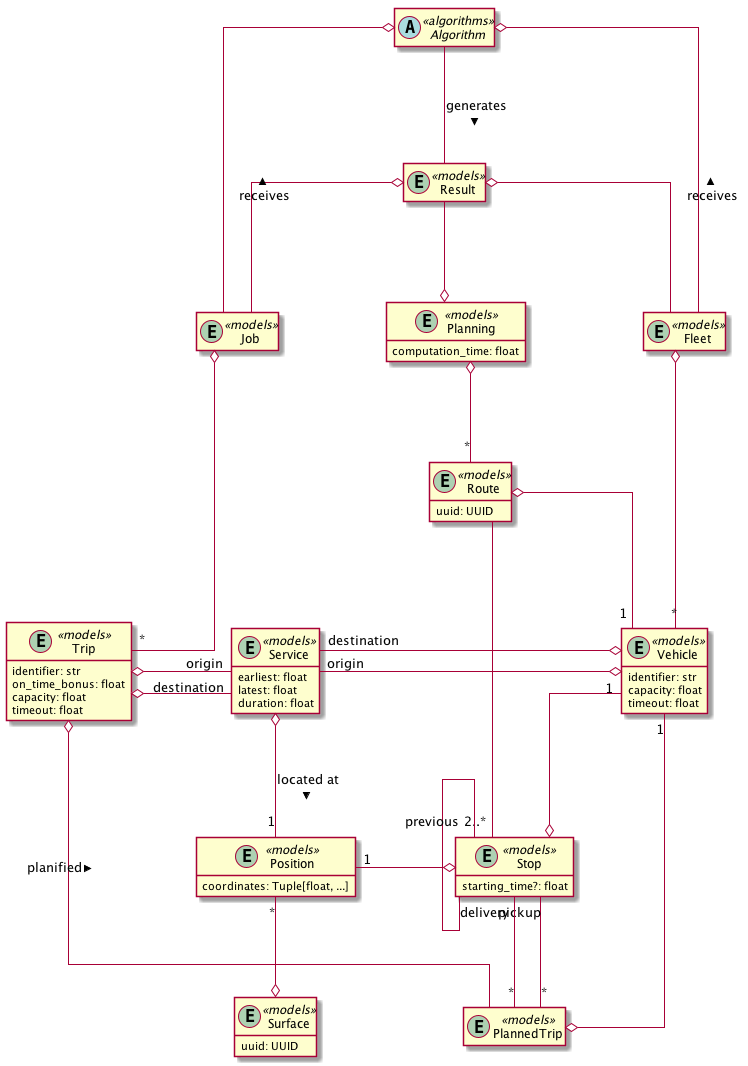
\includegraphics[width=\textwidth]{data-model-overview}
            \caption{Modelo de datos simplificado de la biblioteca \texttt{jinete}.}
            \label{img:data_model_overview}
          \end{figure}

          \paragraph{}
          Siguiendo el mismo orden que el llevado a cabo en el \cref{sec:formulation_keywords}, la primera entidad a comentar es \texttt{Position}, que como su propio nombre indica, se trat de la estructura de datos encargada de modelizar una posición en el espacio. Esto es, aquella que almacena las coordenadas que \say{apuntan} a un determinado punto del espacio. Como es natural, esta es utilizada por el resto de entidades con necesidades de ser localizables en el espacio. En este caso se corresponden con \texttt{Service} (actividad de recogida o entrega relacionada con un viaje) y \texttt{Stop} (acción de moverse hacia un determinado lugar llevada a cabo por un vehículo). Además, para mantener en un contenedor común todas las posiciones surge la entidad \texttt{Surface}.

          \paragraph{}
          La entidad \texttt{Surface} es la encargada de almacenar, proveer e interactuar con entidades \texttt{Position}. Es decir, es la encargada de realizar los cálculos de distancias entre distintos puntos del espacio. Por tanto, tiene la responsabilidad de definir la métrica utilizada en caso de que la distancias sean aritméticas (\emph{Euclídea}, \emph{Manhattan}, etc.) o de calcularlas apoyándose en un servicio cartográfico externo entre otros.

          \paragraph{}
          Siguiendo con las entidades que se encargan de definir las restricciones del problema (posteriormente se continúa con aquellas que recogen el estado y por tanto, el resultado de la optimización) es necesario comentar la labor que desempeña \texttt{Service}. Tal y como se ha dicho anteriormente, esta representa el requisito de llevar a cabo una determinada acción en una determinada posición del espacio. Es decir, es quien contiene información acerca de la ventana temporal disponible para visitar una determinada posición por un vehículo. Además, ofrece la posibilidad de indicar la duración requerida de dicho servicio. Esto es útil para modelar los tiempos de carga y descarga correspondientes. Sin embargo, \texttt{Service} no se utiliza únicamente para representar las tareas de carga y descarga de los viajes. Además, es utilizada para representar el concepto de tiempo de las ventanas temporales de inicio y fin de los vehículos. Es decir, es la manera de representar que un vehículo puede comenzar a operar durante un cierto intervalo de tiempo, y puede volver al almacén en otro determinado intervalo de tiempo. En caso de que ambos puntos sean el mismo, nótese que si dichas ventanas temporales (de comienzo y fin) son disjuntas entonces dicho vehículo estaría obligado a realizar al menos un viaje (lo que puede generar situaciones de infactibilidad de la solución del problema si no hay suficientes viajes disponibles).

          \paragraph{}
          Una de las entidades más importantes desde el punto de vista de la formulación del problema es \texttt{Trip}. Esta es la encargada de \say{conectar} los servicios de recogida y entrega entre si, de tal forma que no puedan ser realizados indistintamente o de manera parcial. Es decir, es quien impone la restricción de que primero se ha de realizar la tarea de visita y, en un tiempo no superior a la duración máxima de viaje, se debe realizar la entrega. Posteriormente, cuando se lleve a cabo la descripción de la entidad \texttt{Stop} se expondrá de manera más detallada cómo es el proceso para llevar esto a cabo. Además de lo indicado, esta es la entidad encargada de indicar la cantidad de espacio (carga) requerido en el vehículo.

          \paragraph{}
          La siguiente entidad a remarcar consiste en \texttt{Job}, cuyo cometido es actuar como un contenedor de viajes (objetos \texttt{Trip}) de tal manera que puedan ser consultados de manera sencilla por otras entidades del modelo de datos. En este caso, \texttt{Job} se corresponde con una visión estática del problema, es decir, no posee ningún conocimiento sobre qué viajes han sido realizados y cuáles no (dicha tarea es responsabilidad de otras entidades).Además de contener todos los viajes del problema, esta también se encarga de contener la entidad \texttt{Objective}, la cual se encarga de representar la función objetivo a optimizar. Esta puede ser de naturaleza muy variada dependiendo de la versión concreta del problema de rutas a resolver. En este trabajo, la más utilizada es la del problema \emph{Dial-a-Ride} por razones obvias, la cual trata de minimizar la distancia total llevada a cabo por los vehículos disponibles.

          \paragraph{}
          Dejando de lado la representación de las necesidades a satisfacer, el siguiente paso es comentar los recursos disponibles para llevarlas a cabo. Como en todos los problemas de rutas, la entidad fundamental que actúa como recurso disponible es la del vehículo. En nuestro caso, dicha función la desempeña \texttt{Vehicle}. En este punto, hay una decisión de diseño importante a tomar, que consiste en la elección entre: \begin{enumerate*}[label=(\alph*)] \item utilizar la entidad vehículo para representar tanto las restricciones que este presenta (tales como capacidad máxima, tiempo máximo de ruta, etc.) como el estado actual (secuencia de tareas o viajes completados, tiempo actual, capacidad actual, etc.) o, por contra, \item dividir dicha entidad en dos, siendo una de ellas la encargada de representar las restricciones anteriormente citadas y otra la encargada de almacenar el estado actual \end{enumerate*}. Como es obvio, cada una una de estas alternativas posee distintas ventajas y desventajas, siendo la primera de ellas más simple pero menos versátil y la segunda, a costa de un mayor grado de complejidad, permite abstraer mejor los conceptos facilitando la implementación de estrategias de optimización avanzadas que requieran de mantener distintas versiones de un mismo vehículo de manera simultanea minimizando la duplicidad de información (y los posibles errores que puedan derivar de dicha situación). En este caso, se ha escogido la segunda opción, por lo que la entidad \texttt{Vehicle} es encargada únicamente de modelizar las restricciones de un vehículo sin mantener constancia de su estado.


          \paragraph{}
          Al igual que se ha indicado para el caso de \texttt{Position} y \texttt{Job}, es necesario añadir una entidad adiccional que actúe como contenedor de estas, siendo \texttt{Surface} y \texttt{Job} respectivamente en los anteriores casos. Por lo tanto, el contenedor de endidades \texttt{Vehicle} se ha denominado \texttt{Fleet} y, al igual que ocurre con \texttt{Job}, su único cometido consiste en proveer de las correspondientes entidades a quien lo requiera. Nótese que el problema \emph{Dial-a-Ride} asume una cantidad finita de vehículos, por lo que esto deberá ser acorde con el funcionamient de \texttt{Fleet}. Sin embargo, existen otros problemas como el \emph{Pickup and Delivery Problem} en que no hay una cota máxima del número de vehículos (a costa de que todos sean iguales entre sí).

          \paragraph{}
          Una vez comentado el significado de todas las entidades de naturaleza estáticas del modelo de datos, el siguiente paso es proceder al razonamiento de las entidades dinámicas, encargadas de almacenar el estado de la optimización. Estas se caracterizan por estar construidas apoyándose en gran medida sobre las anteriores, además de presentar un mayor grado de dificultad tanto en su implementación como explicación por su naturaleza cambiante.

          \paragraph{}
          Siguiendo el orden del \cref{sec:formulation_keywords}, la siguiente entidad a comentar es \texttt{Stop}, cuya función principal es la de representar la realización de un determinado servicio, por un determinado vehículo un estado concreto (posteriormente se indicará cómo se lleva a cabo dicha representación del estado). La entidad \texttt{Stop} se relaciona con el resto de la siguiente manera: con la entidad \texttt{Vehicle} a la cual se refiere, con la entidad \texttt{Position} sobre la cual se localiza, con la entidad \texttt{PlannedTrip} (que se comenta más adelante) sobre la cuál es capaz de relacionarse tanto con el viaje y los servicios requeridos, como con la parada relacionada (de entrega futura si esta es de recogia, o de recogida previa si esta es de entrega). De esta manera es posible verificar si el viaje completo se ha llevado a cabo desde una de las paradas, que no necesariamente tienen por qué ser contiguas entre sí. Adiccionalmente, la entidad \texttt{Stop} incluye otra relación adiccional consigo misma, que representa la anterior parada. De esta manera, todas las paradas de un mismo vehículo están relacionadas entre sí como una lista enlazada. La ventaja de este enfoque es que los cálculos tanto de tiempo como de capacidad actuales, pueden ser calculados desde la propia entidad \texttt{Stop} y la versión anterior de esta generandose una \emph{relación de recurrencia de primer orden}. Por último, esta entidad se relaciona con \texttt{Route}, que como veremos más adelante actúa como contenedor de paradas.

          \paragraph{}
          La siguiente entidad a comentar es \texttt{PlannedTrip}, que como su propio nombre indica se refiere a la realización de un viaje. Esta entidad guarda una \emph{relación fuerte} con las dos paradas necesarias para completar el viaje (la de recogida y la de entrega). Además, esta relacionada con la entidad \texttt{Vehicle} correspondiente.

          \paragraph{}
          Anteriormente se ha indicado que la decisión tomada acerca de cómo representar las restricciones fijas de los vehículos así como su estado actual ha consistido en dividirlo en dos entidades. Ya hemos descrito \texttt{Vehicle}, que es la responsable de definir las restricciones. Sin embargo, todavía no hemos indicado cómo se almacena el estado. Para ello, se ha decidido utilizar la entidad \texttt{Route}, cuyo cometido es almacenar la secuencia de paradas (entidades \texttt{Stop}), y a su vez mantener una relación a través de la cual sea posible recuperar las restricciones de la misma (\texttt{Vehicle}). La ventaja que esta estrategia presenta consiste en la \say{facilidad} para poder mantener varias instancias de la entidad \texttt{Route} referidas al mismo vehículo y al mismo tiempo para que las comparaciones entre estas (para elegir la más beneficiosa para el resultado final) sean mucho más sencillas. Esto es un factor importante en la resolución de este tipo de problemas donde la carga computacional derivada de la evaluación combinatoria es muy elevada.

          \paragraph{}
          La última entidad a comentar consiste en \texttt{Planning}, la cuál actúa como un contenedor de entidades \texttt{Route}. Tal y como se ha comentado antes, estas se refieren a la secuencia de paradas para cada vehículo. Nótese que deben satisfacer la restricción de que  un vehículo tan solo tenga una ruta a realizar por razones obvias. Lo interesante de esta entidad es que es la utilizada como valor de entrada y salida para muchos de los métodos de resolución implementados (entidades \texttt{Algorithm}), lo cual permite que estos puedan ser intercambiados y combinados entre sí fácilmente.

          \paragraph{}
          Tal y como se puede apreciar a lo largo del apartado, el modelado del problema de manera adecuada se ha correspondido con una tarea de gran peso para la implementación realizada. A lo largo de la descripción, se ha tratado de comentar la taxonomia definida manteniendo el equilibrio adecuado entre detalle y extensión del mismo, dejando de lado algunos detalles técnicos de menor relevancia para la visión general del modelo de datos.

        \subsubsection{Carga de Datos}
        \label{sec:implementation_components_data_loading}

          \paragraph{}
          El proceso de carga de datos en la implementación llevada a cabo consiste más concretamente en la lectura de los valores concretos que definen las diferentes instancias del problema a resolver, los cuales consisten en el número de viajes requeridos así como las características concretas de cada uno de ellos, o los vehículos disponibles para satisfacer dichos viajes, con sus corresponientes limitaciones tanto de tiempo como de carga.

          \paragraph{}
          [TODO]

          \begin{figure}[h]
            \centering
            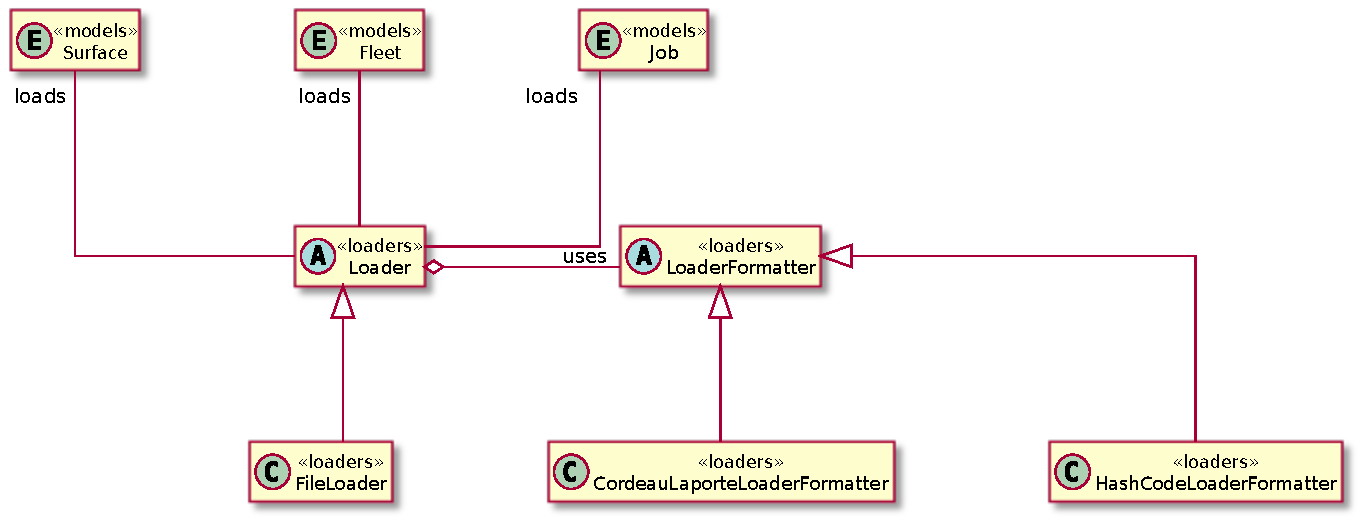
\includegraphics[width=\textwidth]{loaders-overview}
            \caption{Diagrama de clases del módulo \texttt{loaders} perteneciente a la biblioteca \texttt{jinete}.}
            \label{img:loaders_overview}
          \end{figure}

          \paragraph{}
          [TODO]

          \paragraph{}
          [TODO]

        \subsubsection{Optimización del Problema}
        \label{sec:implementation_components_optimization}

          \paragraph{}
          [TODO]

          \begin{sidewaysfigure}[h]
            \centering
            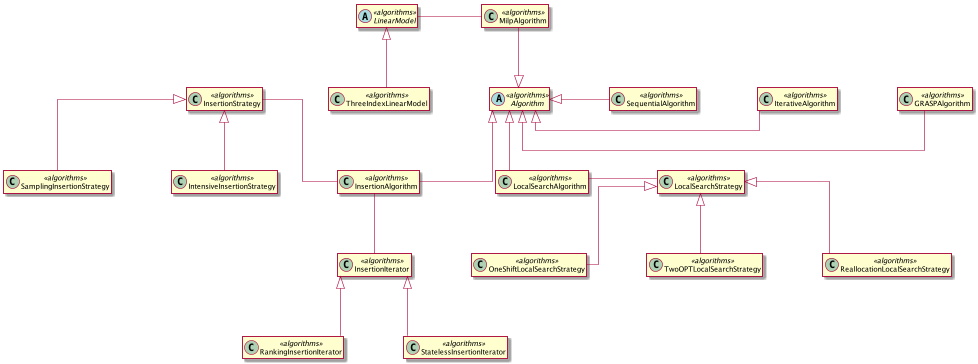
\includegraphics[width=\textwidth]{algorithms-overview}
            \caption{Diagrama de clases del módulo \texttt{algorithms} perteneciente a la biblioteca \texttt{jinete}.}
            \label{img:algorithms_overview}
          \end{sidewaysfigure}

          \paragraph{}
          [TODO]

        \subsubsection{Exportación de Resultados}
        \label{sec:implementation_components_exportation}

          \paragraph{}
          [TODO]

          \begin{figure}[h]
            \centering
            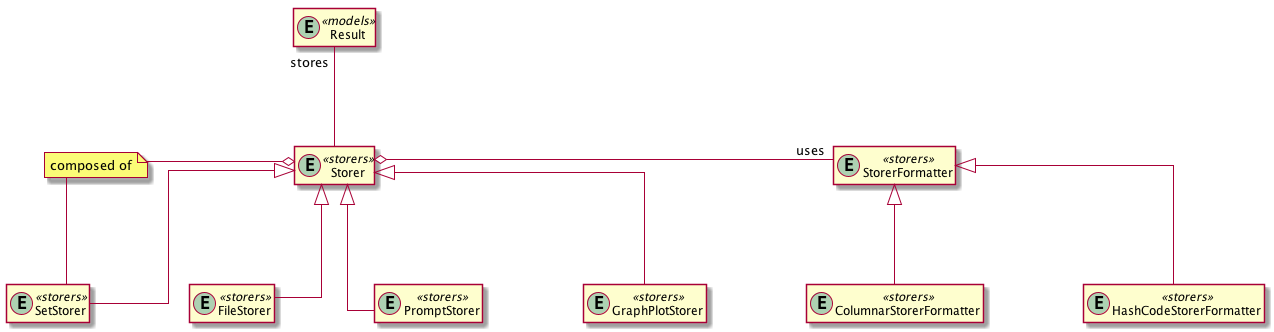
\includegraphics[width=\textwidth]{storers-overview}
            \caption{Diagrama de clases del módulo \texttt{storers} perteneciente a la biblioteca \texttt{jinete}.}
            \label{img:storers_overview}
          \end{figure}

          \paragraph{}
          [TODO]

    \section{Resultados}
    \label{sec:results}

      \paragraph{}
      [TODO]

      \subsection{Definición del experimento}
      \label{sec:results_definition}

        \paragraph{}
        [TODO]

      \subsection{Tablas de resultados}
      \label{sec:results_tables}

        \paragraph{}
        [TODO]

      \subsection{Análisis de resultados}
      \label{sec:results_analysis}

        \paragraph{}
        [TODO]

    \section{Conclusiones}
    \label{sec:implementation_results_conclusions}

      \paragraph{}
      [TODO]

\end{document}
